\chapter{Progettazione della Soluzione}

\section{Class Diagram del dominio della soluzione}
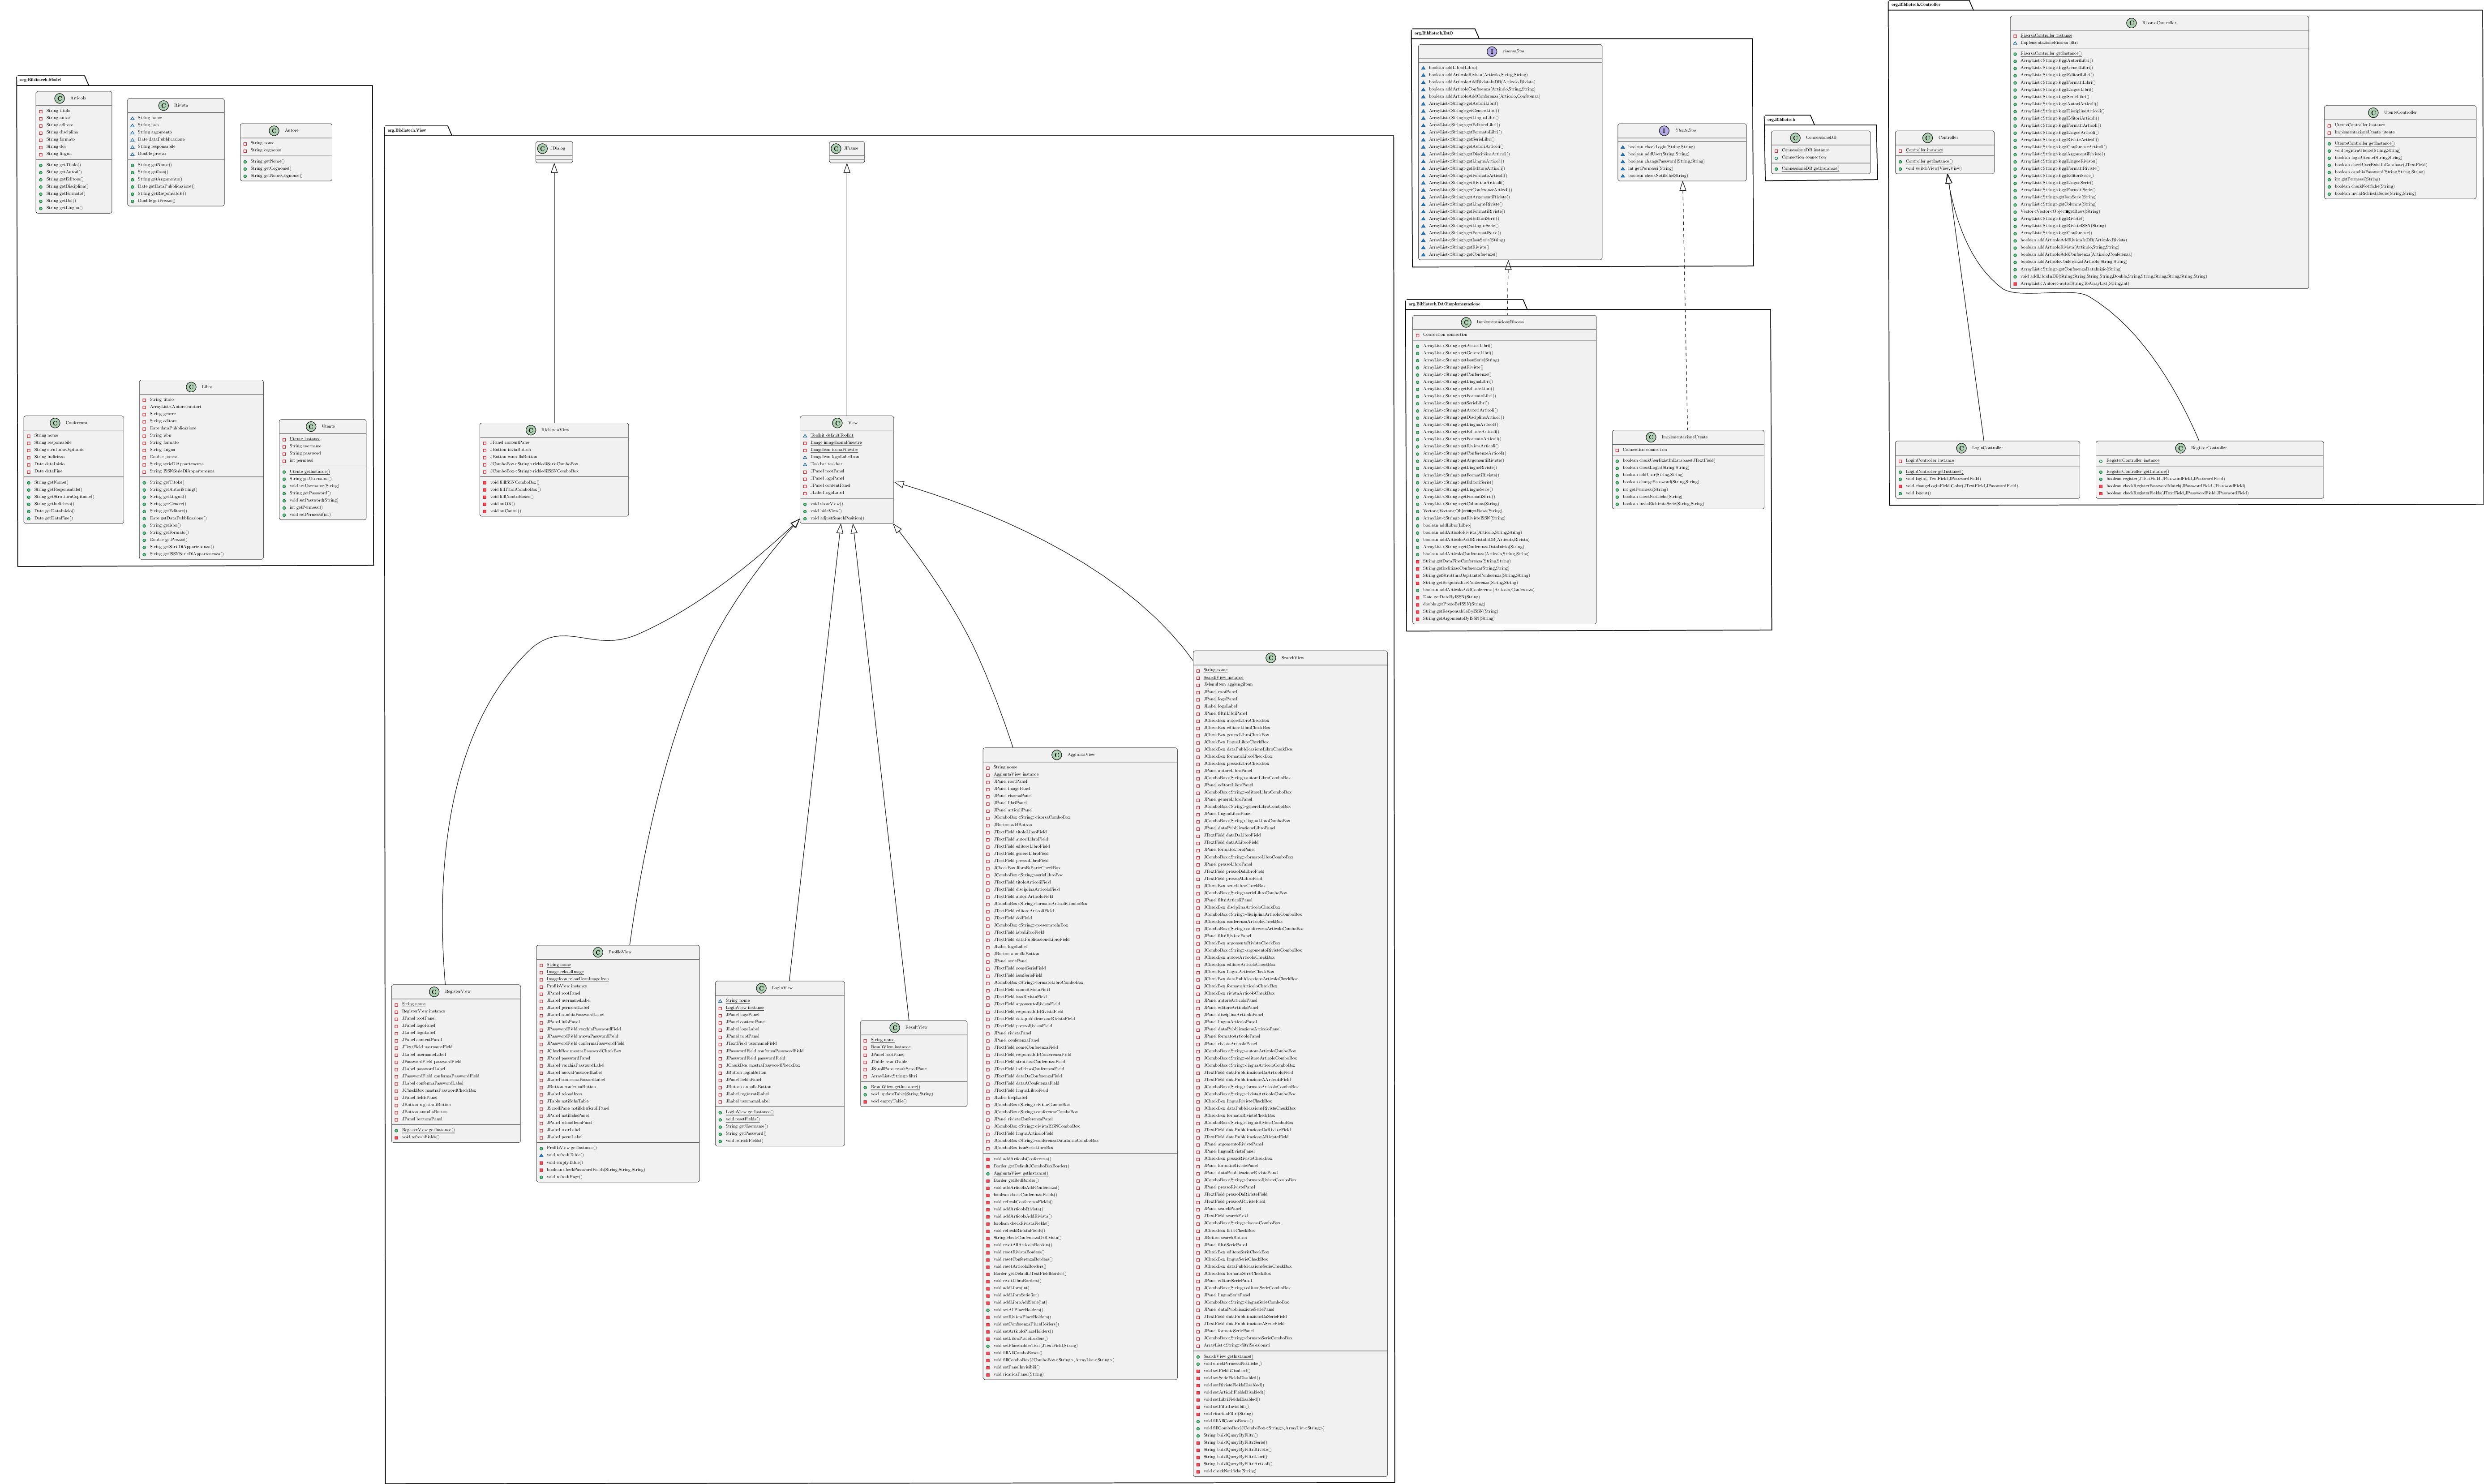
\includegraphics[scale=0.05, center]{Immagini/PDiagram.png}

\subsection{Dizionario dei Metodi}
\begin{longtable}{|l|l|}
    \hline
    Classe             & Metodi                                                                                                                                                                                                                                                                                                                                                      \\ \hline
    \endhead
    Controller         & +void switchView()                                                                                                                                                                                                                                                                                                                                          \\ \hline
    UtenteController   & \begin{tabular}[c]{@{}l@{}}+ void registraUtente()\\ + boolean loginUtente()\\ + boolean checkUserExistInDatabase()\\ + boolean cambiaPassword()\\ + int getPermessi()\\ + boolean checkNotifiche()\\ + boolean inviaRichiestaSerie()\end{tabular}                                                                                                          \\ \hline
    LoginController    & \begin{tabular}[c]{@{}l@{}}+ void login(JPasswordField)\\ - void changeLoginFieldsColor()\\ + void logout()\end{tabular}                                                                                                                                                                                                                                    \\ \hline
    RegisterController & \begin{tabular}[c]{@{}l@{}}+ boolean register()\\ - boolean checkRegisterPasswordMatch()\\ - boolean checkRegisterFields()\end{tabular}                                                                                                                                                                                                                     \\ \hline
    RisorsaController  & \begin{tabular}[c]{@{}l@{}}+ boolean addArticoloAddRivistaInDB()\\ + boolean addArticoloRivista()\\ + boolean addArticoloAddConferenza()\\ + boolean addArticoloConferenza()\\ + ArrayList\textless{}String\textgreater getConferenzaDataInizio()\\ + void addLibroInDB()\\ - ArrayList\textless{}Autore\textgreater autoriStringToArrayList()\end{tabular} \\ \hline
    View               & \begin{tabular}[c]{@{}l@{}}+ void showView()\\ + void hideView()\\ + void adjustSearchPosition()\end{tabular}                                                                                                                                                                                                                                               \\ \hline
    Articolo           & \begin{tabular}[c]{@{}l@{}}+ String getTitolo()\\ + String getAutori()\\ + String getEditore()\\ + String getDisciplina()\\ + String getFormato()\\ + String getDoi()\\ + String getLingua()\end{tabular}                                                                                                                                                   \\ \hline
    Rivista            & \begin{tabular}[c]{@{}l@{}}+ String getNome()\\ + String getIssn()\\ + String getArgomento()\\ + Date getDataPubblicazione()\\ + String getResponsabile()\\ + Double getPrezzo()\end{tabular}                                                                                                                                                               \\ \hline
    Autore             & \begin{tabular}[c]{@{}l@{}}+ String getNome()\\ + String getCognome()\\ + String getNomeCognome()\end{tabular}                                                                                                                                                                                                                                              \\ \hline
    Conferenza         & \begin{tabular}[c]{@{}l@{}}+ String getNome()\\ + String getResponsabile()\\ + String getStrutturaOspitante()\\ + String getIndirizzo()\\ + Date getDataInizio()\\ + Date getDataFine()\end{tabular}                                                                                                                                                        \\ \hline
    Libro              & \begin{tabular}[c]{@{}l@{}}+ String getTitolo()\\ + String getAutoriString()\\ + String getLingua()\\ + String getGenere()\\ + String getEditore()\\ + Date getDataPubblicazione()\\ + String getIsbn()\\ + String getFormato()\\ + Double getPrezzo()\\ + String getSerieDiAppartenenza()\\ + String getISSNSerieDiAppartenenza()\end{tabular}             \\ \hline
    \end{longtable}

\section{Sequence Diagram del metodo addArticoloConferenza}
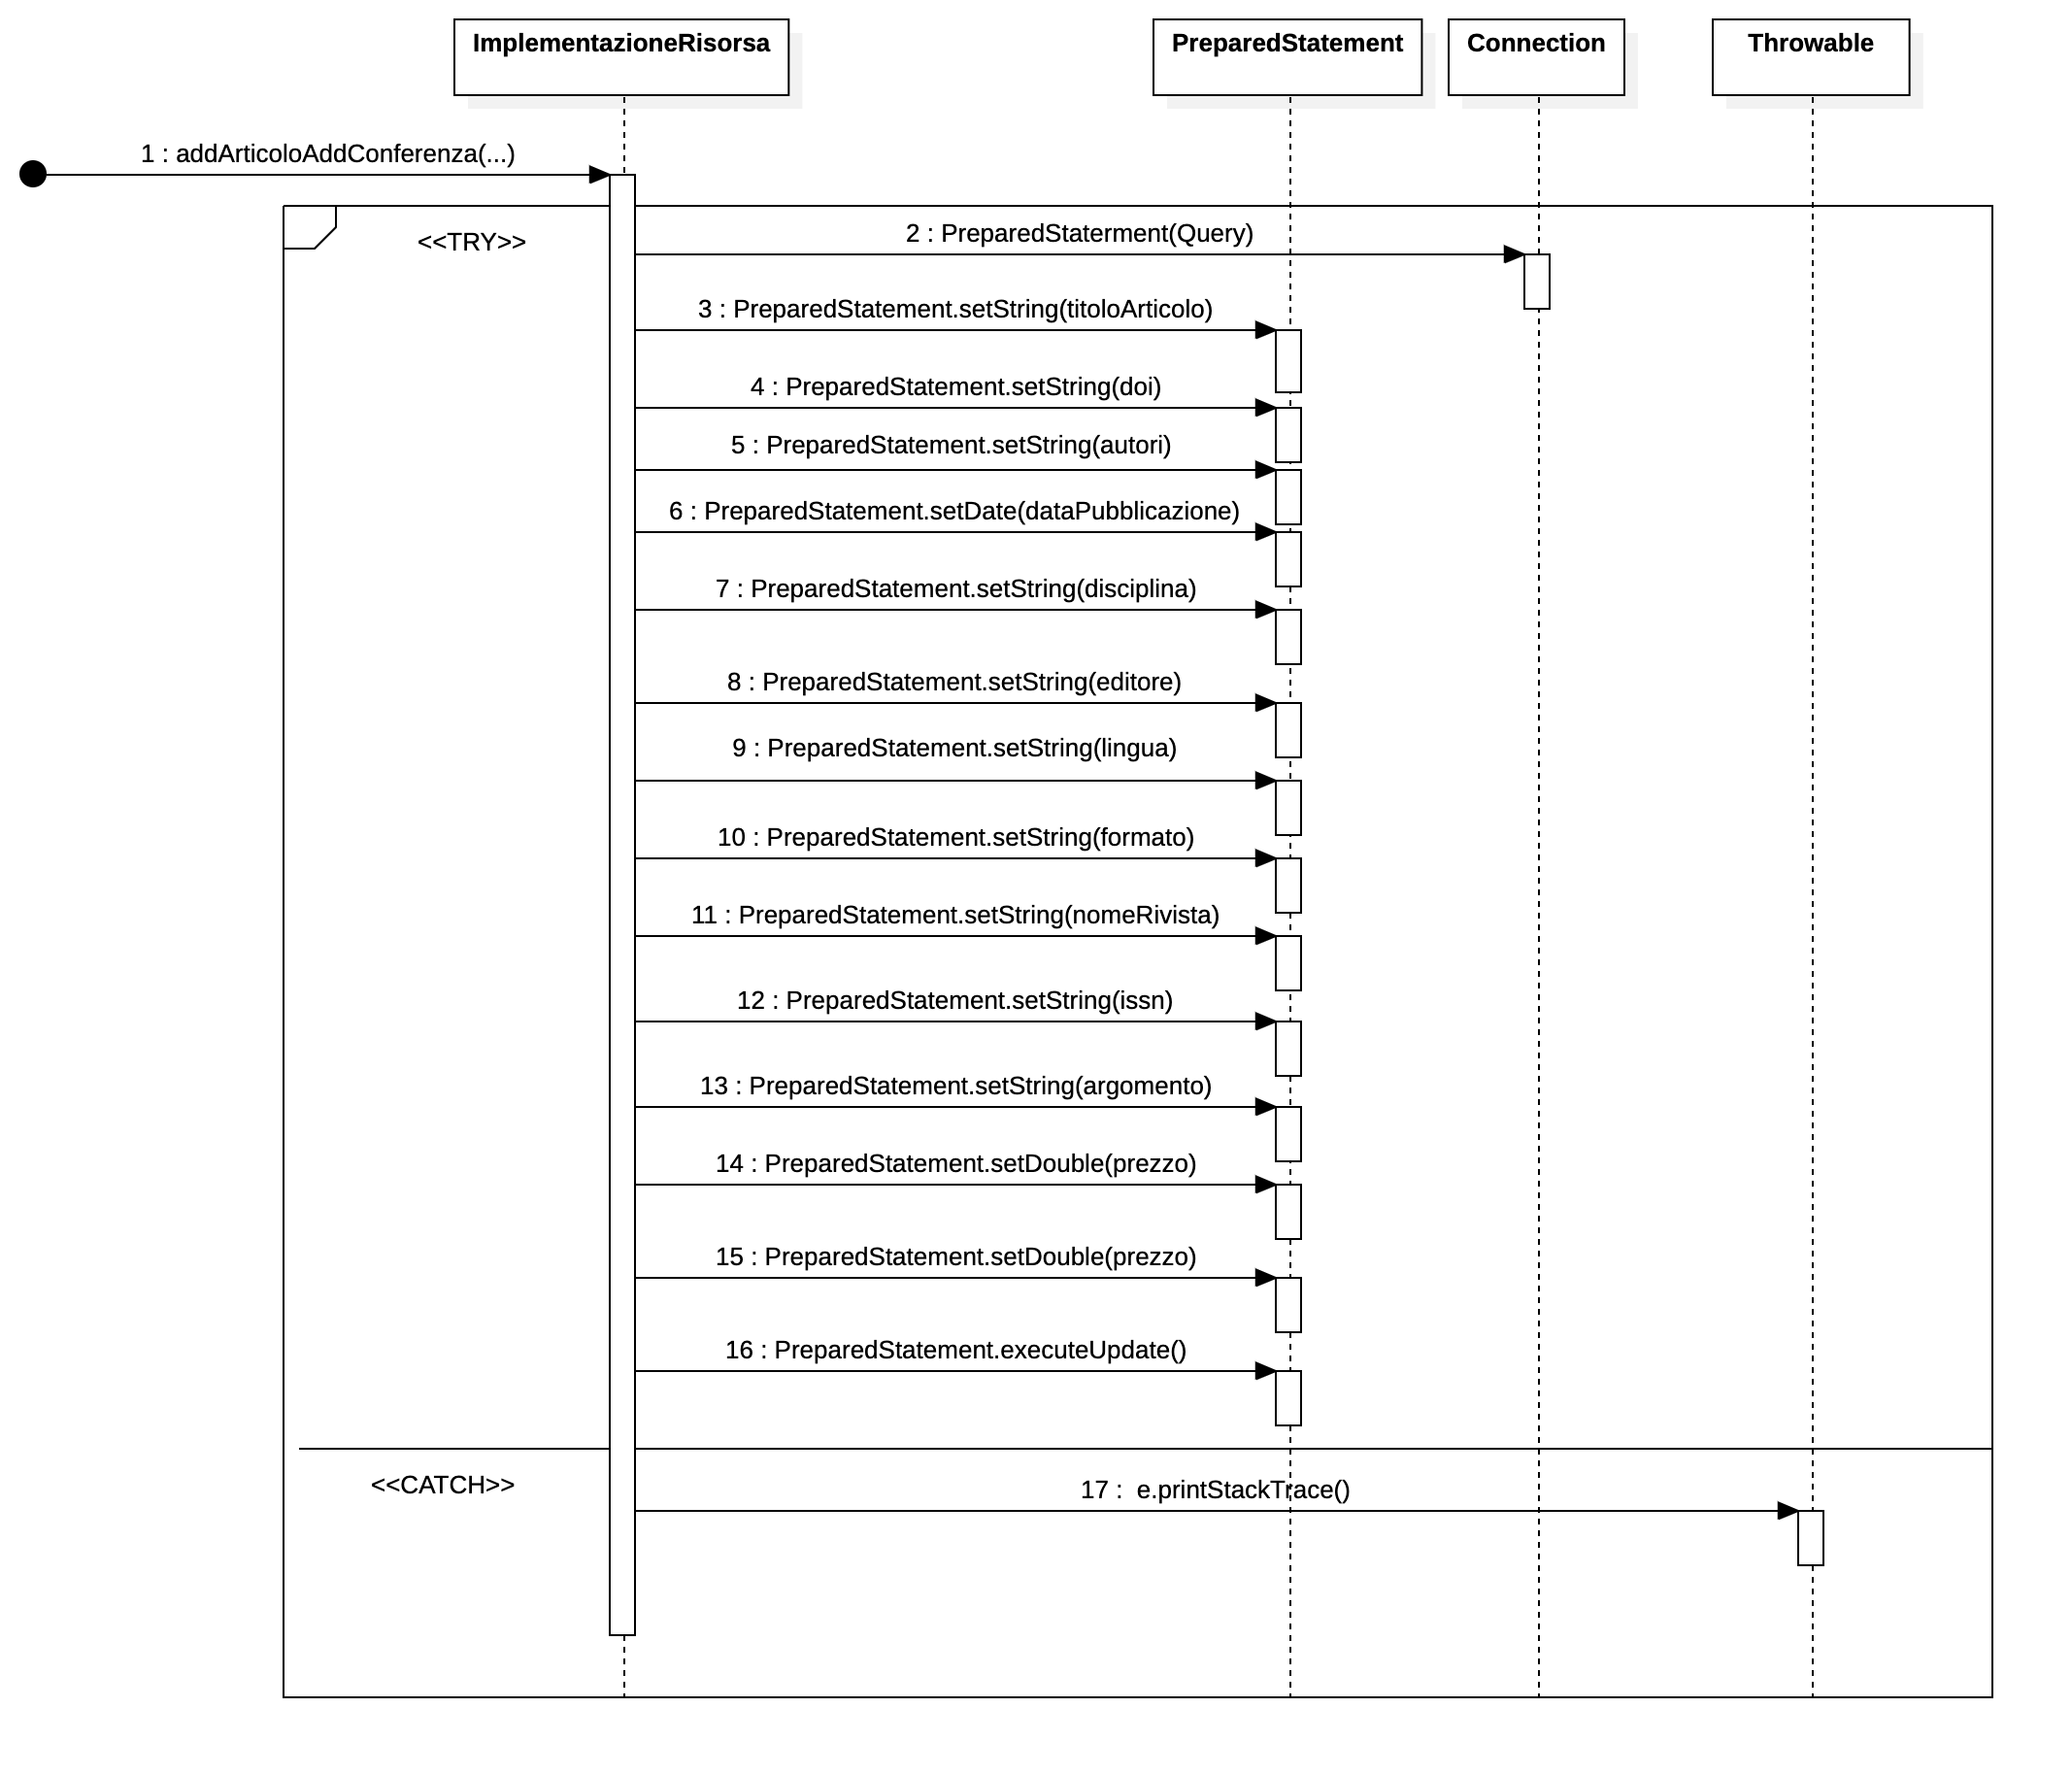
\includegraphics[scale=0.15, center]{Immagini/AddArtConf_SD.png}

\section{Sequence Diagram del metodo checPermessiNotifiche}
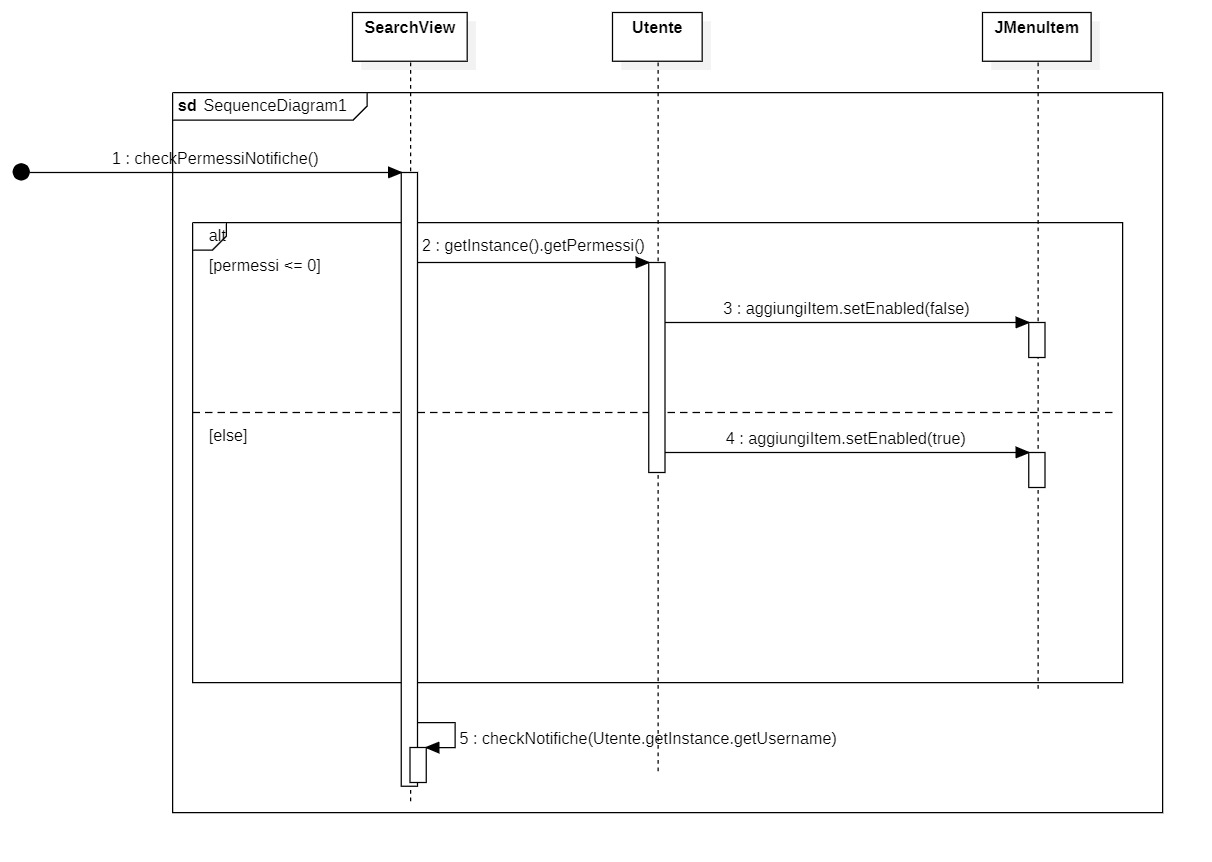
\includegraphics[scale=0.28, center]{Immagini/checkPermNot_SD.jpg}
